\chapterimage{capitulos.pdf}
\chapter{\emph{Gartner Scores}}
\label{anexo-tabelacc}

%A próxima página apresenta tabela\footnote{A tabela original do \relatorioGCC \xspace é chamada de ``\emph{Table 2: Product/Service Rating on Critical Capabilities}.''} contendo a atribuição de notas (\emph{scores}) para cada fornecedor avaliado (horizontal) para cada uma das 15 áreas de capacidade (vertical). 

A próxima página apresenta tabela elaborada a partir do \relatorioGCC contendo a atribuição de notas (\emph{scores}) para cada fornecedor avaliado (horizontal) de cada uma das 15 áreas de capacidade (vertical).

As notas variam de $1,0$ a $5,0$ e apresentam o seguinte significado:

\begin{itemize}
    \item \textbf{1 = Fraco ou ausente}: a maioria ou todos os requisitos definidos para uma capacidade não são alcançados;   
    \item \textbf{2 = Regular}: alguns requisitos não são alcançados;
    \item \textbf{3 = Bom}: atende aos requisitos;
    \item \textbf{4 = Excelente}: atende ou excede alguns requisitos;   
    \item \textbf{5 = Excelente}: excede significativamente os requisitos;
\end{itemize}

Os resultados dos casos de uso construídos no ``\autoref{cap-casos-gartner} -- \nameref{cap-casos-gartner}'' da ``\autoref{parte-estudosdecaso} -- \nameref{parte-estudosdecaso}'' são obtidos pela soma da multiplicação dos pesos definidos para cada área de capacidade e as notas atribuídas a cada fornecedor de acordo com essa tabela. 
\thispagestyle{empty}
\begin{landscape}
    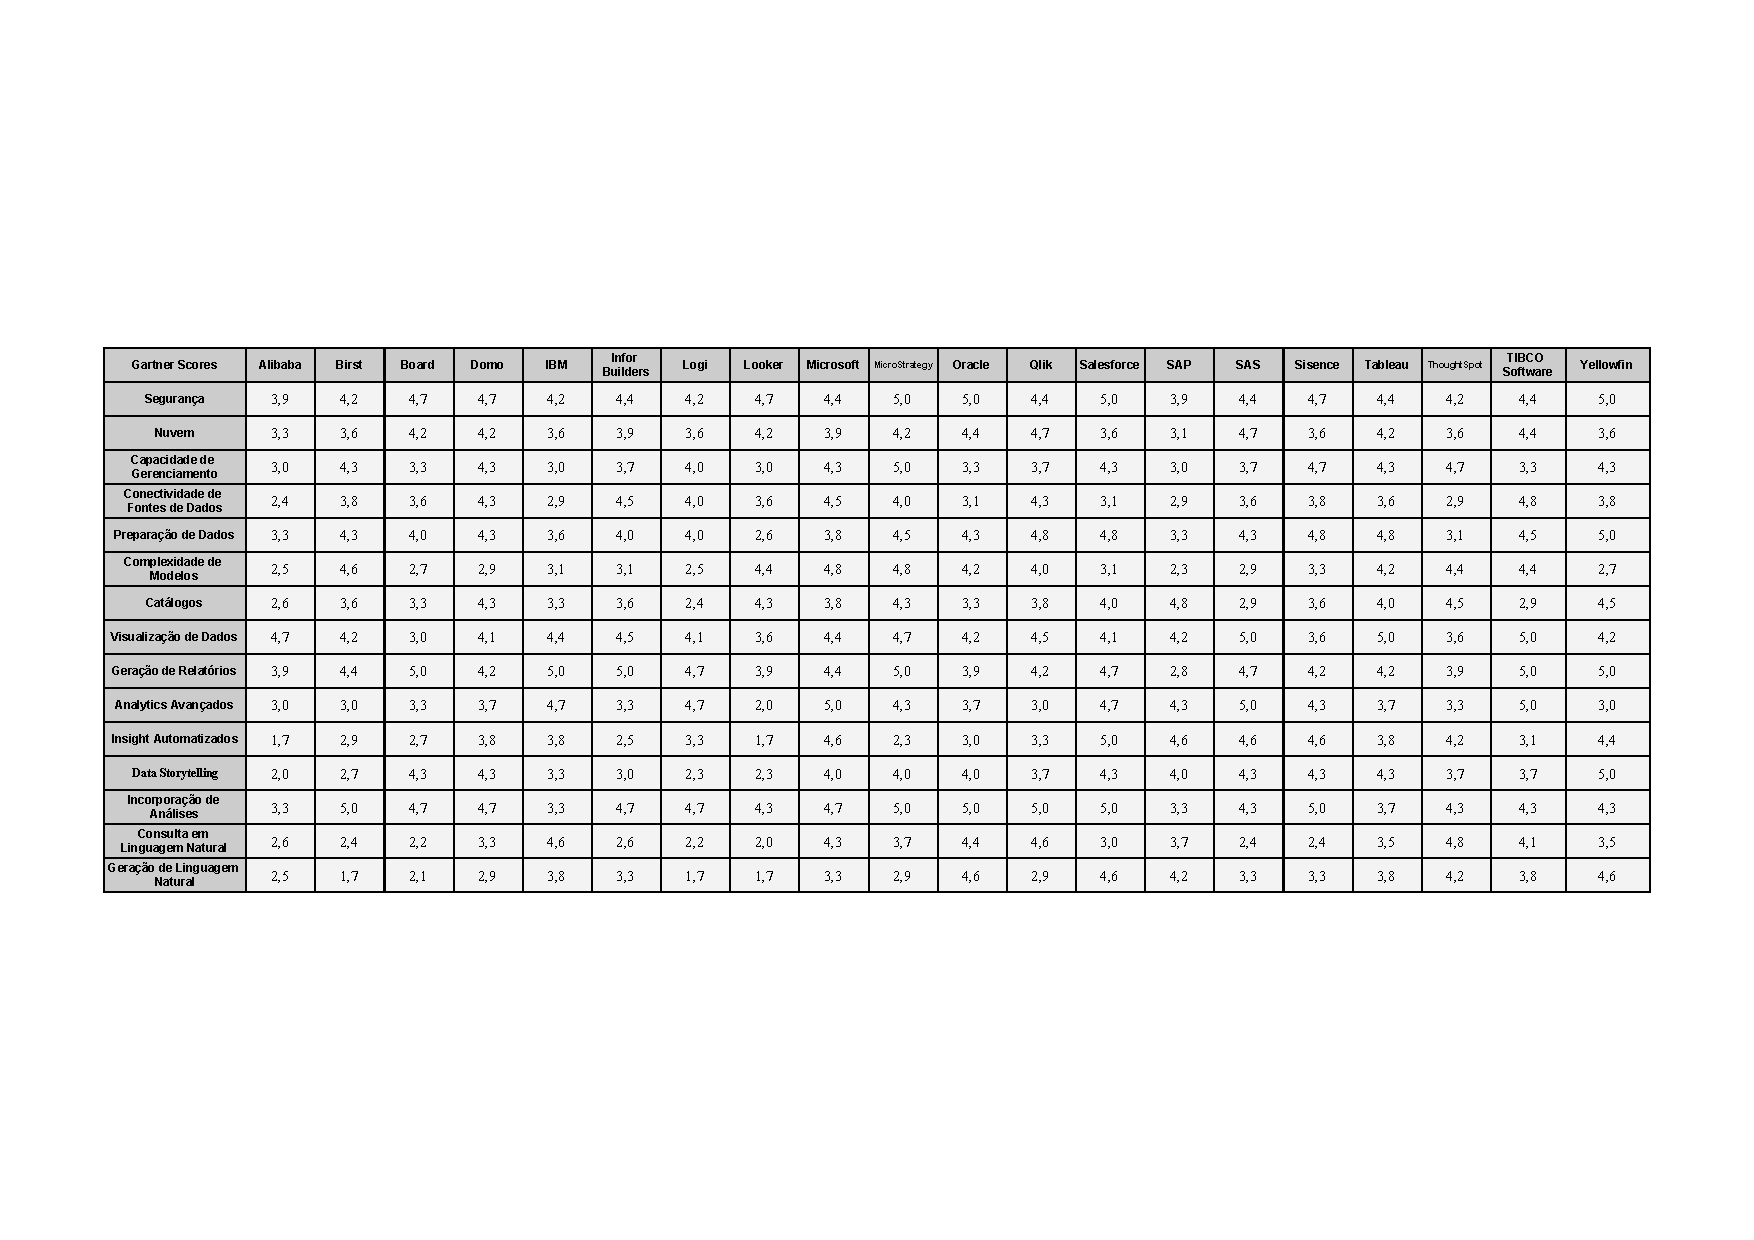
\includepdf[pages=-,angle=90]{gartner.pdf}
\end{landscape}